\documentclass{beamer}
\usepackage{fontspec}
%\usepackage[T2A]{inputenc}
%\usepackage{tikz}
%\usepackage{multicol}
%\usepackage{amsmath}
%\setmainfont{DejaVu Serif}
\usepackage[serbian]{babel}
\setmainfont{FreeSerif}
\usepackage{graphicx}
\usepackage{listings}
\usepackage{adjustbox}
\usetheme{Berlin}

\title{Problem rotacije useva}
\author{Nikola Šutić}
\date{12.5.2024}

\begin{document}

%\logo{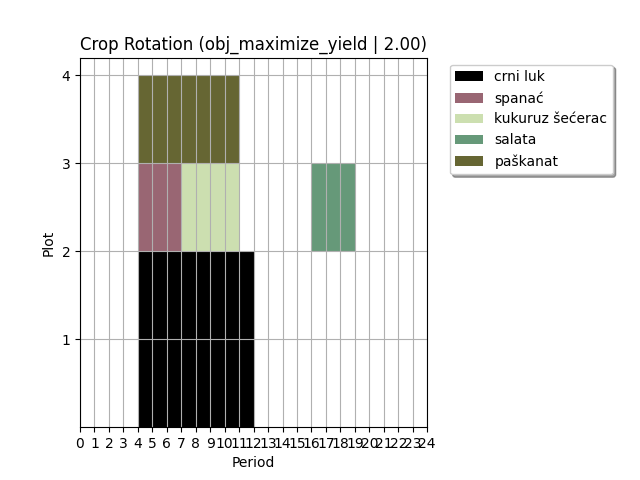
\includegraphics[width=0.33\textwidth]{slike/yield.png}}

\frame{\titlepage}

\begin{frame}
  \frametitle{Uvod}
  
  \begin{itemize}
  \item{Koncept rotacije useva}
  \item{Potreba za rotacijom useva}
  \item{Problem sa ručnim planiranjem}
  \end{itemize}
\end{frame}

\begin{frame}
  \frametitle{Principi}

  \begin{itemize}
  \item{Rotacija useva: principi, benefiti, izazovi}
  \item{Genetski algoritam: koncept, postuptak i prilagođenje problemu useva}
  \end{itemize}
\end{frame}

\begin{frame}
  \frametitle{Postavka problema}

  \begin{itemize}
  \item{Optimizacija rotacije useva}
  \item{Faktori koji utiču: nutrienti zemljišta, upravljanje bolestima i napastima, klima, prinos itd.}
  \end{itemize}
\end{frame}

\begin{frame}
  \frametitle{Metodologija}

  \begin{itemize}
  \item{Opis algoritma - inicijalizacija, ukrštanje, odabir roditelja, fitnes jedinke, mutacija}
  \item{Prilagođavanje problema algoritmu}
  \item{Ograničenja}
  \end{itemize}
  
\end{frame}

\begin{frame}

  \frametitle{Implementacija i delovi koda}

  \begin{figure}
    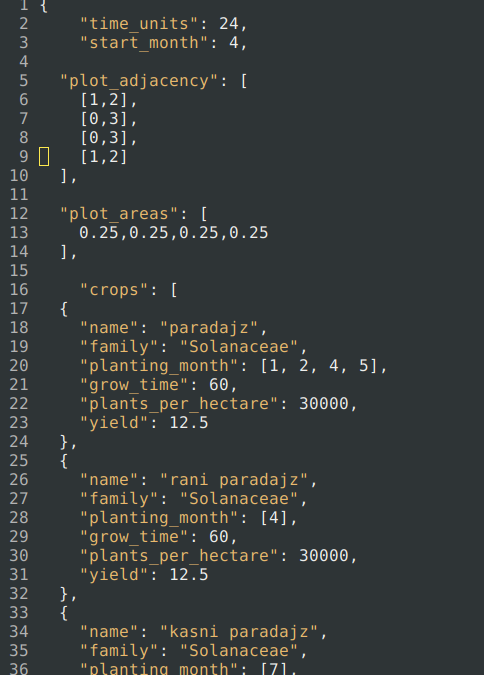
\includegraphics[height=0.7\textheight]{slike/problem_spec.png}
    \caption{Specifikacija konkretne instance problema CR}
  \end{figure}
  %\begin{lstlisting}
  %  import numpy
  %  asdads
  %  asdas
  %\end{lstlisting}

\end{frame}
\begin{frame}

  \frametitle{Implementacija i delovi koda}

  \begin{figure}
    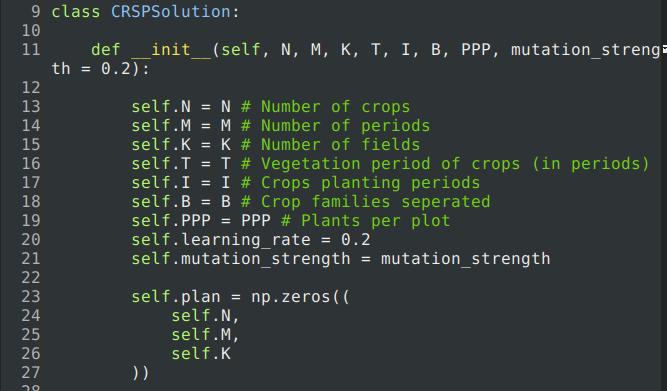
\includegraphics[height=0.7\textheight]{slike/CRSPSolution.png}
    \caption{Implementacija jedinke}
  \end{figure}
  %\begin{lstlisting}
  %  import numpy
  %  asdads
  %  asdas
  %\end{lstlisting}

\end{frame}
\begin{frame}

  \frametitle{Implementacija i delovi koda}

  \begin{figure}
    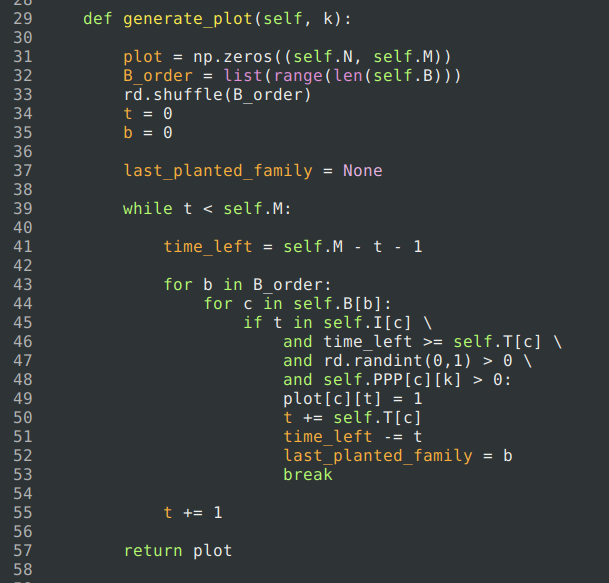
\includegraphics[height=0.7\textheight]{slike/generate_plot.png}
    \caption{Generisanje mogućeg poretka za jedno parče zemljišta}
  \end{figure}
  %\begin{lstlisting}
  %  import numpy
  %  asdads
  %  asdas
  %\end{lstlisting}

\end{frame}
\begin{frame}

  \frametitle{Implementacija i delovi koda}

  \begin{figure}
    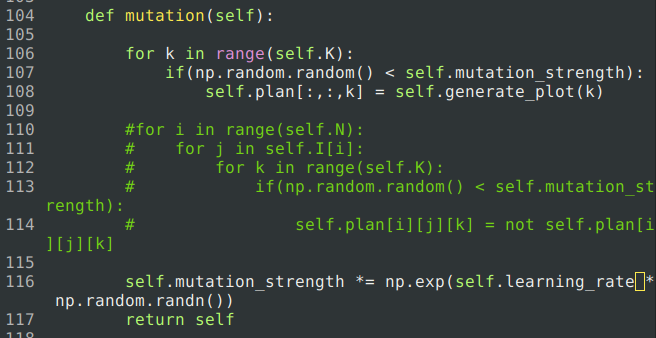
\includegraphics[height=0.7\textheight]{slike/mutation.png}
    \caption{Mutacijom uvodimo novi redosled za jedno parče zemlje}
  \end{figure}
  %\begin{lstlisting}
  %  import numpy
  %  asdads
  %  asdas
  %\end{lstlisting}

\end{frame}

\begin{frame}[fragile]
  \frametitle{Implementacija i delovi koda}

  \begin{lstlisting}[language=Python]
      def fitness(self, sol):

        _fitness = self.objective(sol) +\
                   self.constraint2(sol) +\
                   self.constraint3(sol) +\
                   self.constraint4(sol) +\
                   self.constraint5(sol) +\
                   self.constraint6(sol) +\
                   self.constraint7(sol) +\
                   self.constraint8(sol)
  \end{lstlisting}
\end{frame}

\begin{frame}

  \frametitle{Implementacija i delovi koda}

  \begin{figure}
    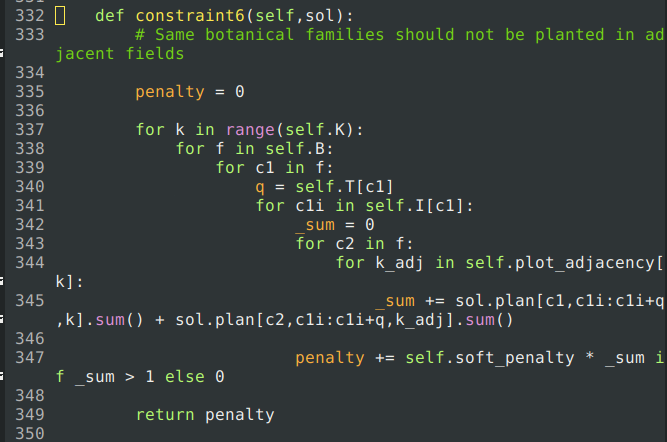
\includegraphics[height=0.7\textheight]{slike/constraint6.png}
    \caption{Primer jednog ograničenja (Iste porodice biljaka ne smeju biti jedna pored druge)}
  \end{figure}
  %\begin{lstlisting}
  %  import numpy
  %  asdads
  %  asdas
  %\end{lstlisting}

\end{frame}

\begin{frame}
  \frametitle{Rezultat i diskusija}
  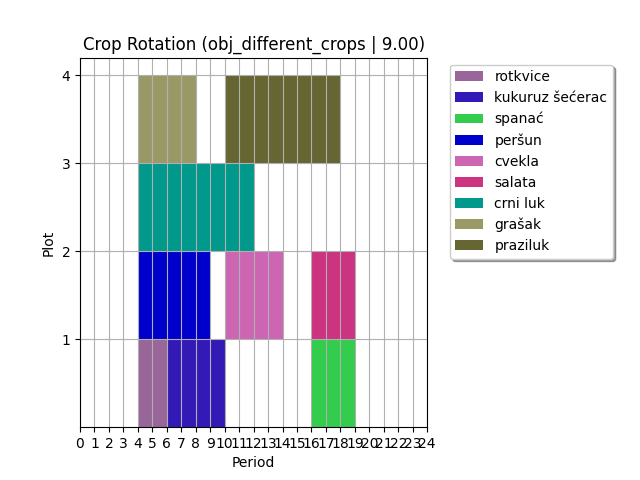
\includegraphics[height=0.85\textheight]{slike/diverse.png}
\end{frame}
\begin{frame}
  \frametitle{Rezultat i diskusija}
  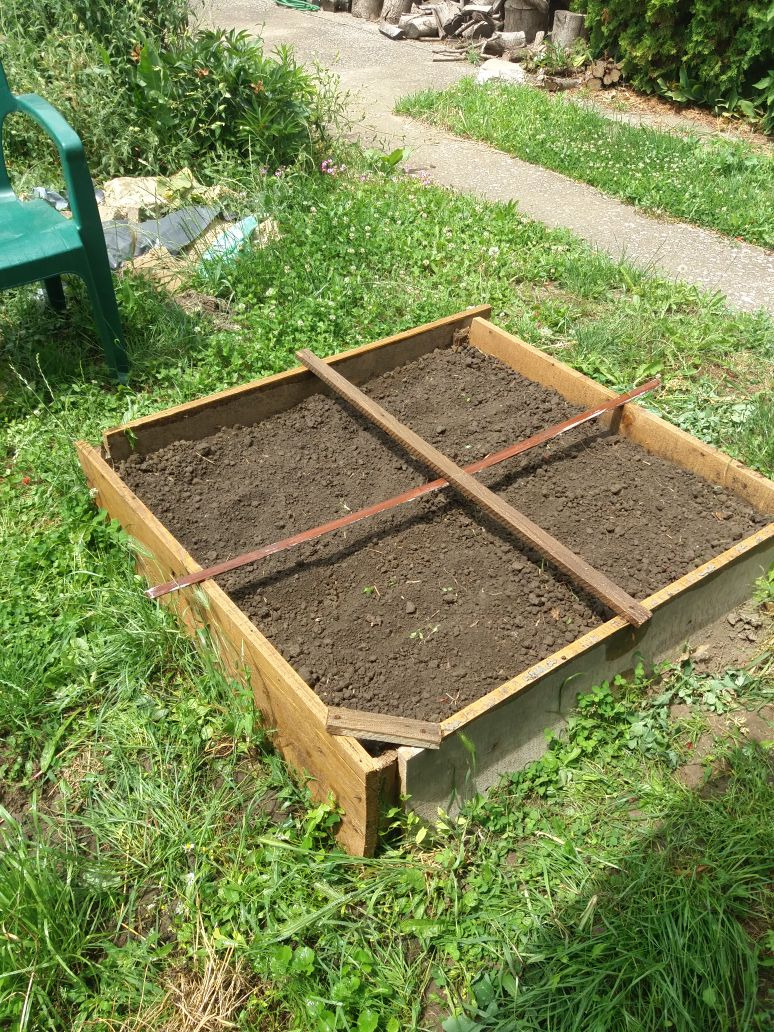
\includegraphics[height=0.85\textheight]{slike/basta3}\centering
\end{frame}
\begin{frame}
  \frametitle{Rezultat i diskusija}
  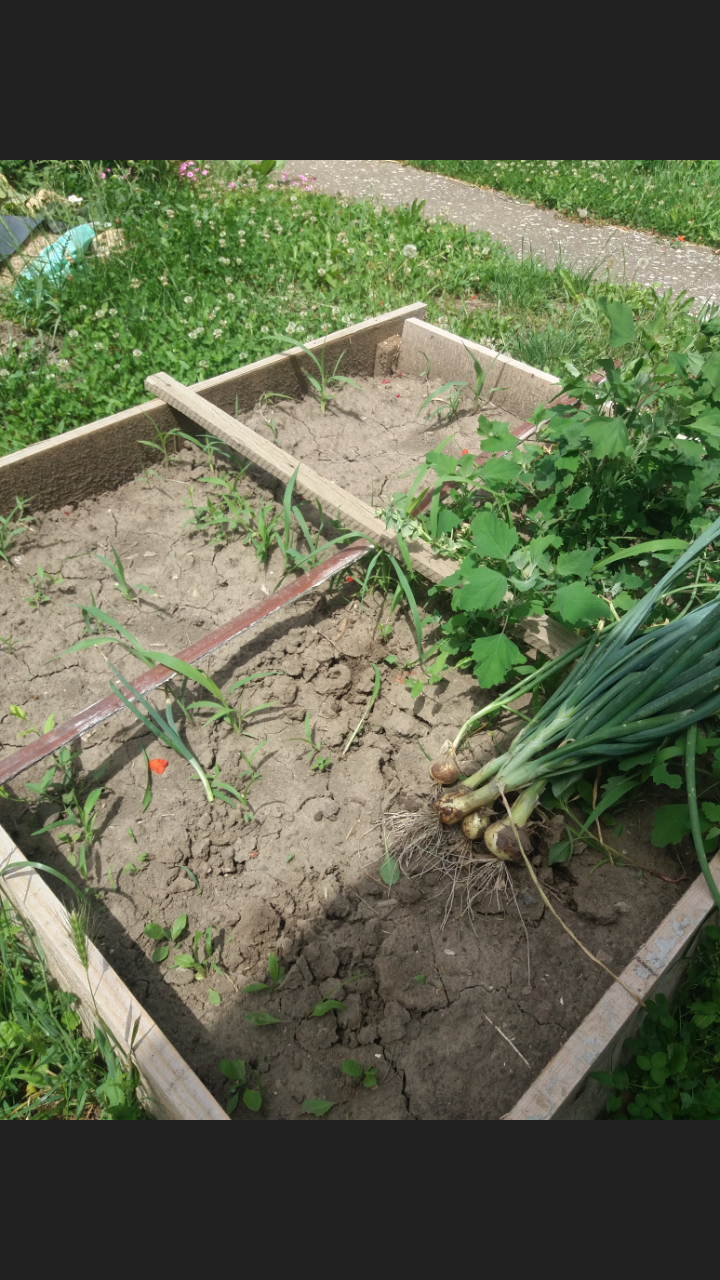
\includegraphics[height=0.85\textheight]{slike/basta2}\centering
\end{frame}
\begin{frame}
  \frametitle{Rezultat i diskusija}
  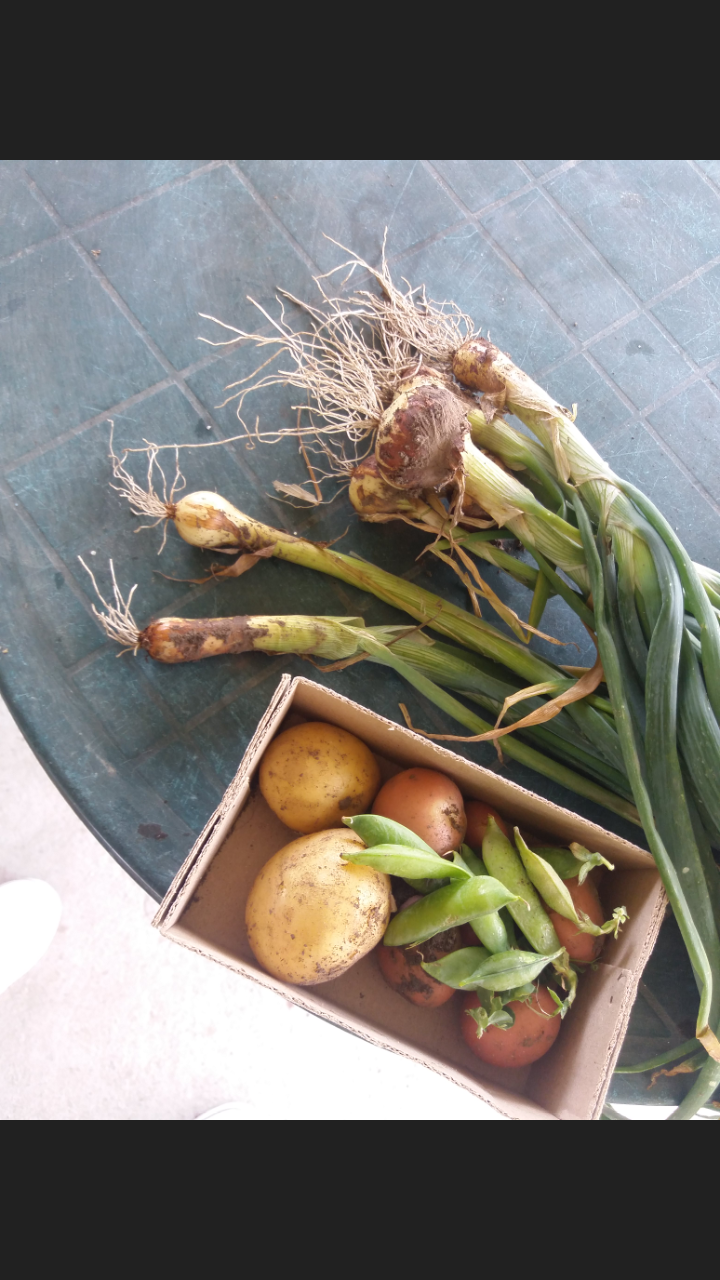
\includegraphics[height=0.85\textheight]{slike/basta1}\centering
\end{frame}
\begin{frame}
  \frametitle{Rezultat i diskusija}
  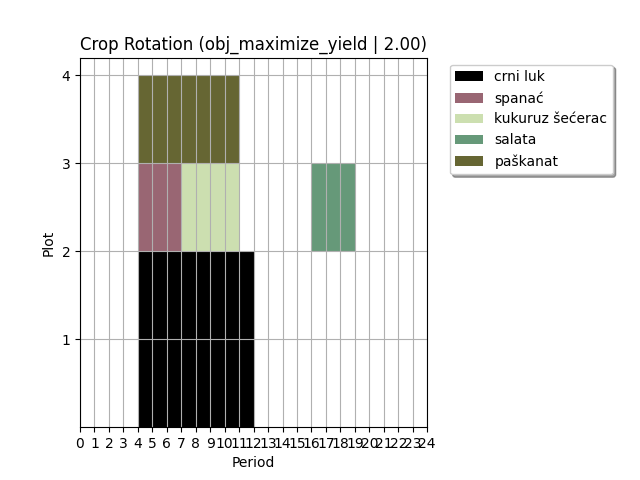
\includegraphics[height=0.85\textheight]{slike/yield.png}
\end{frame}

\begin{frame}
  \frametitle{Ograničenja i dalji rad}

  \begin{itemize}
  \item{\textbf{Dostupnost podataka u poljoprivredi}}
  \item{Veliki broj matematičkih ograničenja}
  \item{Učenje potkrepljivanjem}
  \end{itemize}
\end{frame}

\begin{frame}
  \frametitle{Zaključak}

  \begin{itemize}
  \item{Problem, rešenje, rezultat}
  \item{Primena naprednih optimizacionih algoritama u polju poljoprivrede}
  \end{itemize}
\end{frame}

\end{document}
